\documentclass[norsk,a4paper,12pt]{article}
\usepackage[utf8]{inputenc}  %æøå
\usepackage{graphicx} %for å inkludere grafikk
\usepackage{verbatim} %for å inkludere filer med tegn LaTeX ikke liker
\usepackage{tabularx}
\usepackage{booktabs}
\usepackage{float}
\usepackage{color}
\usepackage{listings}
\usepackage{hyperref}

\title{FYS2160 - Termodynamikk\\\vspace{2mm} \Large{Labøvelse 1 - Faseoverganger}}
\author{\large \"Omer Faruk \"Ozt\"urk\\ Stian B. S{\o}isdal\\ Even Marius Nordhagen}
\date{\today}
\begin{document}
\maketitle

\section{Hensikt}
Hensikten med dette forsøket er at vi skal få en dypere forståelse av hvordan varmekapasiteten til et kalorimeter henger sammen med forskjellige parameter for et varmeelement, og hvordan den spesifikke smeltevarmen igjen henger sammen med denne varmekapasiteten, den spesifikke varmekapasiteten til vann og forskjellige temperaturer (som vi vil gå nærmere inn på senere). Vi skal også bli kjent med Clausius-Clapeyrons likning og ved hjelp av denne beregne vannets fordampningsvarme.\par\vspace{5mm}

Som indikert ovenfor, består dette forsøket av to delforsøk hvor det første går ut på å beregne smeltevarmen til vann ved hjelp av målinger og matematiske relasjoner. Den andre delen går ut på å beregne vannets fordampningsvarme. Av denne grunn vil alle kategorier være delt inn i to deler som tar for seg de to hoveddelene ved forsøket.

\section{Apparatur}
\subsection{Smeltevarme}
For å beregne smeltevarme trenger vi følgende apparater
\begin{itemize}
\item Kalorimeter
\item Strømforsyning
\item Amperemeter
\item Voltmeter
\item Termometer (PASCO, koblet til PC via USB)
\item Digitalvekt
\item Isblokk i et isvannbad (kar med is og vann)
\item Datamaskin med datalogger
\end{itemize}

\subsection{Fordampningsvarme}
For å beregne fordampningsvarme trenger vi følgende utstyr
\begin{itemize}
\item Kolbe ($A$)
\item Glassrør
\item Gummislange
\item Buffervolum ($B$)
\item Vannstrålepumpe
\item Varmeelement
\item Manometer (trykksensor)
\item To haner ($H_1$ og $H_2$)
\item Kokstein
\end{itemize}
Alle benevninger som står i parantes er knyttet til Figur (\ref{fig:fordampningsvarme}) og er brukt på samme måte som i figuren.
\begin{figure}[H]
\centering
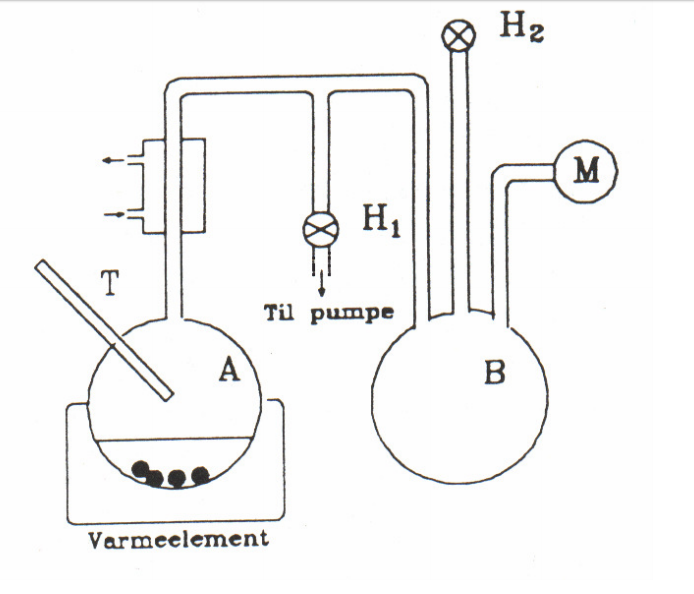
\includegraphics[width=120mm]{fordampningsvarme.png}
\caption{Oppsett for måling av relevante faktorer når man skal beregne fordampningsvarmen til vann.}
\label{fig:fordampningsvarme}
\end{figure}

\section{Fremgangsmåte}
\subsection{Beregning av smeltevarme}
Det første vi skal gjøre er å beregne smeltevarmen $L_s$ ved hjelp av formel (\ref{eq:latentheat}), noe vi trenger parameterene $C_0$, $C_v$, $m$, $T_0$, $T_1$ og $T_2$ til. 
\begin{equation}
m\Big[L_s+C_v(T_2-T_0)\Big] = C_0(T_1-T_2)
\label{eq:latentheat}
\end{equation}
Massen til isen som blir smeltet i kalorimeteret $m$, vannets spesifikke varmakapasitet $C_v$ og temperaturen $T_0$ har vi generelle verdier for, mens de øvrige er vi nødt til å beregne gjennom målinger.\par
$C_0$ kan finnes ved formelen
\begin{equation}
C_0\bigg(\frac{dT}{dt}\bigg)=U\cdot I
\end{equation}
hvor vi setter strømmen lik $I=0.75A$, måler spenningen over varmeelementet med et multimeter og beregner $dT/dt$ ut fra et kalorimeter fylt med 1.25 liter vann med temperatur som øker fra $20^o$C til $30^o$C.\par
Vi er nå klare til å gjøre målinger direkte knyttet til smeltevarmen. Det første vi gjør, er å smelte en isklump i kalorimeteret mens temperaturen logges. Ut fra dette kan vi finne temperaturene $T_1$ og $T_2$.

\subsection{Beregning av fordampningsvarme}
For å beregne smeltevarmen, må vi bruke Clausius-Clapeyrons likning
\begin{equation}
\ln\frac{P_1}{P_2}=-\frac{L_f}{R}\bigg(\frac{1}{T_1}-\frac{1}{T_2}\bigg)
\end{equation}
hvor $R$ er konstant, mens $L_f$ er den molare fordampningsvarmen, som vi skal finne. Vi må beregne damptrykkene $P_1$ og $P_2$ ved temperaturene $T_1$ og $T_2$, noe som gjøres når systemet er i en stasjonær tilstand, siden metningstrykket over vanndampen (som vi måler) da er likt trykket i vannet. Vi måler temperaturen i vannet. 

\section{Måledata}
Under målingen av smeltevarme var spenningsfallet over varmeelementet konstant på ca ...V. Temperaturøkningen var på $10^o$C, og det tok ... sekunder å gjennomføre denne endringen.\par 
Vi fant så at temperaturene var
\begin{equation}
T_1=...,\quad\quad T_2=...
\end{equation}
ved trykkene
\begin{equation}
P_1=...,\quad\quad P_2=...
\end{equation}
for en isklump som veier ...

\section{Resultat}
Vi fant at 
\begin{equation}
\frac{dT}{dt}=\frac{10^oC}{...s}=...
\end{equation}
Dette gir kalorimeteret en spesifikk varmekapasitet på:
\begin{equation}
C_0=U\cdot I\bigg(\frac{dT}{dt}\bigg)^{-1}=
\end{equation}
Vi kan løse Formel (\ref{eq:latentheat}) med hensyn på den latente varmekapasiteten, og vi får den til å være:
\begin{equation}
L_s=\frac{C_0(T_1 - T_2)}{m}-C_v(T_2 - T_0)=\frac{C_0(T_1 - T_2)}{m}J/kg-4200(T_2)J/kg=
\end{equation}
\emph{\color{red} Må forklare formelen ovenfor (Oppgave 3)}\newline
Den molare fordampningsvarmen er gitt ved
\begin{equation}
L_f=R\ln\bigg(\frac{P_1}{P_2}\bigg)\bigg(\frac{T_1T_2}{T_1-T_2}\bigg)
\end{equation}
hvor konstanten $R=k_BN_A$, hvor $k_B$ igjen er Boltzmanns konstant og $N_A$ er Avogadros tall. Vi er ute etter fordampningsvarmen per masse (ikke per mol), og fra en kjemisk tabell over molare masser kan man finne at den molare massen til vann (og is) er $18 g/mol$. Fordampningsvarmen per gram er derfor
\begin{equation}
L_f=18\cdot6.022\cdot10^{23}\cdot1.381\cdot10^{-23}\ln\bigg(\frac{P_1}{P_2}\bigg)\bigg(\frac{T_1T_2}{T_1-T_2}\bigg)J/g
\end{equation}
\emph{\color{red} Må svare på spørsmål 6}
\end{document}